\newcommand{\NWtarget}[2]{\hypertarget{#1}{#2}}
\newcommand{\NWlink}[2]{\hyperlink{#1}{#2}}
\newcommand{\NWtxtMacroDefBy}{Fragment defined by}
\newcommand{\NWtxtMacroRefIn}{Fragment referenced in}
\newcommand{\NWtxtMacroNoRef}{Fragment never referenced}
\newcommand{\NWtxtDefBy}{Defined by}
\newcommand{\NWtxtRefIn}{Referenced in}
\newcommand{\NWtxtNoRef}{Not referenced}
\newcommand{\NWtxtFileDefBy}{File defined by}
\newcommand{\NWtxtIdentsUsed}{Uses:}
\newcommand{\NWtxtIdentsNotUsed}{Never used}
\newcommand{\NWtxtIdentsDefed}{Defines:}
\newcommand{\NWsep}{${\diamond}$}
\newcommand{\NWnotglobal}{(not defined globally)}
\newcommand{\NWuseHyperlinks}{}
% -*- mode: latex; coding: utf-8 -*-

\documentclass[%
    a4paper,    % Use A4, not US letter!
    justified,  % Use justified text
    nobib,      % Disable natbib
    openany     % Remove blank pages used for two page layout
]{tufte-book}

% -*- mode: latex; coding: utf-8 -*-

% Load packages
% ---------------------------------------------------------------------------
\usepackage[usenames,dvipsnames,svgnames]{xcolor}
\usepackage{minted}
\usepackage[english]{babel}              % English hyphenation
\usepackage[utf8]{inputenc}              % UTF-8 input encoding
% \usepackage[T1]{fontenc}                 % hyphenation of words with ä,ö and ü
\usepackage{booktabs,tabularx}           % package for nicer tables
\usepackage{pgfgantt}                    % Provides GANTT charts
\usepackage[owncaptions]{vhistory}       % Provides framework for creating history outline
\usepackage{csquotes}                    % Quotes
\usepackage{nameref}                     % Allows referencing of names
\usepackage{blindtext}                   % Dummy text
\usepackage[pages=some]{background}            % Backgrounds
\usepackage[absolute,overlay]{textpos}
\usepackage{hyperref}
\usepackage{makeidx}
\usepackage[nonumberlist,nomain]{glossaries}
\usepackage{todonotes}
\usepackage[
    backend=biber,
    style=ieee,
    sortlocale=de_DE,
    natbib=true,
    url=false, 
    doi=true,
    eprint=false
]{biblatex}
\usepackage{bookmark}
\usepackage{esvect}                          % Provides nicer vector display in math mode
\usepackage[inline]{enumitem}
\usepackage{tikz}
\usepackage{float}
\usepackage{cleveref}

% Settings
%---------------------------------------------------------------------------
% TIKZ: A lot of arrows for TIKZ
\usetikzlibrary{arrows.meta}

% TUFTE: Do not break when there already is a break
% Source: https://tex.stackexchange.com/questions/291746/tufte-latex-newthought-after-section
\makeatletter
\def\tuftebreak{%
  \if@nobreak\else
    \par
    \ifdim\lastskip<\tufteskipamount
      \removelastskip \penalty -100
      \tufteskip
    \fi
  \fi
}
\makeatother

% Environments
% ---------------------------------------------------------------------------
\newenvironment{loggentry}[2]% date, heading
{\noindent\textbf{#1}\marginnote{#2}\\}

% Commands
%---------------------------------------------------------------------------
% Prints the month name (e.g., January) and the year (e.g., 2008)
% -*- mode: latex; coding: utf-8 -*-

\newcommand{\monthyear}{%
  \ifcase\month\or January\or February\or March\or April\or May\or June\or
  July\or August\or September\or October\or November\or
  December\fi\space\number\year
}

% Definition of colors
%---------------------------------------------------------------------------
% -*- mode: latex; coding: utf-8 -*-

\definecolor{linkblue}{rgb}{0,0,0.8}       % Standard
\definecolor{darkblue}{rgb}{0,0.08,0.45}   % Dark blue
\definecolor{bfhgrey}{rgb}{0.41,0.49,0.57} % BFH grey
\definecolor{linkcolor}{rgb}{0,0,0}
\colorlet{Black}{black}
\definecolor{keywords}{rgb}{255,0,0}
\definecolor{red}{rgb}{0.6,0,0}
\definecolor{green}{rgb}{0,0.5,0}
\definecolor{blue}{rgb}{0,0,0.5}
% Syntax colors
\definecolor{syntaxRed}{rgb}{0.6,0,0}
\definecolor{syntaxBlue}{rgb}{0,0,0.5}
\definecolor{syntaxComment}{rgb}{0,0.5,0}
% Background colors
\definecolor{titlepagecolor}{cmyk}{1,.60,0,.40}
\definecolor{syntaxBackground}{rgb}{0.95, 0.95, 0.95}

% (Code-) Listings
%---------------------------------------------------------------------------
% -*- mode: latex; coding: utf-8 -*-

\newminted{python}{%
    bgcolor=LightGray,
    escapeinside=||,
    linenos=true,
    mathescape=true,
}

% Generate index
%---------------------------------------------------------------------------
\makeindex

% Global variables
%---------------------------------------------------------------------------
\newcommand{\titletext}{QDE.}
\newcommand{\subtitletext}{A system for composing real time computer graphics.}
\newcommand{\subsubtitletext}{MTE7103 --- Master thesis}
\author[Sven Osterwalder]{Sven Osterwalder}
\publisher{Berne University of Applied Sciences}

% Commands
%----------------------------------------------------------------------------
\renewcommand\labelenumi{(\theenumi)}

% Background set up
%---------------------------------------------------------------------------
\backgroundsetup{
    scale=1,
    angle=0,
    opacity=1,
    contents={
        \begin{tikzpicture}[remember picture,overlay]
            \node[anchor=south west, inner sep=0pt,outer sep=0pt] at (current page.south west) {%
                \includegraphics[width=1.0\paperwidth,height=0.5\paperheight]{images/bg}
            };
        \end{tikzpicture}
    }
}
\makeatletter
\def\printauthor{%
    {\large \@author}}
\makeatother

% Set up bibliography
%----------------------------------------------------------------------------
\addbibresource{inc/bibliography.bib}
\DefineBibliographyStrings{ngerman}{
    andothers = {{et\,al\adddot}},
}

\begin{document}

% Title Page and Abstract
%---------------------------------------------------------------------------
\setcounter{page}{1}
% -*- mode: latex; coding: utf-8 -*-

\begin{titlepage}
    \BgThispage
    \begin{fullwidth}%
        \sffamily%
        \fontsize{36}{40}\selectfont\par\noindent\textcolor{darkgray}{\allcaps{\titletext{}}}
        \vspace{3mm}
        \fontsize{18}{20}\selectfont\par\noindent\textcolor{darkgray}{\allcaps{\subtitletext{}}}
        \vspace{6mm}
        \fontsize{14}{16}\selectfont\par\noindent\allcaps{\subsubtitletext{}}%
        \vspace{24mm}
        \normalsize\normalfont%
        \begin{tabbing}
        xxxxxxxxxxxxxxx \= xxxxxxxxxxxxxxxxxxxxxxxxxxxxxxxxxxxxxxxxxxxxxxx \kill
        Major:          \> Computer science                              \\
        Author:         \> Sven Osterwalder\protect\footnotemark[1]{}    \\
        Advisor:        \> Prof.~Claude Fuhrer\protect\footnotemark[2]{} \\
        Expert:         \> Dr.~Eric Dubuis\protect\footnotemark[3]{}     \\
        Date:           \> \vhCurrentDate{}                              \\
        Version:        \> \vhCurrentVersion                             \\
        \end{tabbing}
        \vspace{10mm}
        \begin{tabularx}{0.5\textwidth}{@{}XX@{}}
            \includegraphics[width=50px]{images/by-sa-big} & 
            \includegraphics[height=20pt]{images/BFH_Logo_B} \\

            \tiny{\sffamily{This work is licensed under
            a~\href{http://creativecommons.org/licenses/by-sa/4.0/}{Creative
            Commons Attribution-ShareAlike 4.0 International
            License}.}}\index{license}
            & \tiny{\sffamily{Berne University of Applied Sciences}}\\
        \end{tabularx}
        \footnotetext[1][-10pt]{sven.osterwalder@students.bfh.ch}
        \footnotetext[2]{claude.fuhrer@bfh.ch}
        \footnotetext[3]{eric.dubuis@comet.ch}
    \end{fullwidth}%
\end{titlepage}
\restoregeometry
\thispagestyle{empty}%
\clearpage%

% -*- mode: latex; coding: utf-8 -*-

% Versions:
% -----------------------------------------------

\chapter*{}
\label{chap:versions}

\begin{versionhistory}
    \vhEntry{ 89c7544 }{ 2017-02-28 17:09:43 }{ SO }{ Set up initial project structure, provide first content }
    \vhEntry{ 10192d8 }{ 2017-03-02 22:37:17 }{ SO }{ Set up project schedule }
    \vhEntry{ 54f4b23 }{ 2017-03-05 22:53:15 }{ SO }{ Set up project structure, implement main entry point and main window }
    \vhEntry{ ffda0e5 }{ 2017-03-15 10:58:51 }{ SO }{ Scene graph, logging, adapt project schedule }
    \vhEntry{ 34b09b7 }{ 2017-03-24 17:08:22 }{ SO }{ Update meeting minutes, thoughts about node implementation }
    \vhEntry{ 06fe268 }{ 2017-04-03 23:00:35 }{ SO }{ Add requirements, node graph implemenetation }
    \vhEntry{ d264175 }{ 2017-04-10 16:07:01 }{ SO }{ Conversion from Org-Mode to Nuweb, revise editor implementation }
    \vhEntry{ f8b524b }{ 2017-04-30 23:42:57 }{ SO }{ Approach node graph and nodes }
    \vhEntry{ 2f46832 }{ 2017-05-04 21:13:41 }{ SO }{ Impel node definitions further }
    \vhEntry{ ae34fc5 }{ 2017-05-24 13:56:31 }{ SO }{ Change class to tufte-book, title page, introduction, further implementation }
    \vhEntry{ 27c549c }{ 2017-05-24 22:28:41 }{ SO }{ Change document structure, re-work admin. aspects }
    \vhEntry{ 6772ef9 }{ 2017-05-27 14:18:09 }{ SO }{ Adapt document structure, fundamentals: introduction and rendering }
    \vhEntry{ 399669d }{ 2017-05-29 09:10:48 }{ SO }{ Finish fundamentals }
    
\end{versionhistory}% -*- coding: utf-8 -*-

\chapter*{Abstract}
\label{chap:abstract}

\todo[inline]{Provide correct abstract.}
A highly optimized rendering algorithm based on ray
tracing is presented. It outperforms the classical ray tracing methods and
allows the rendering of ray traced scenes in real-time on the GPU.~The
classical approach for modelling scenes using triangulated meshes is replaced
by mathematical descriptions based on signed distance functions. The
effectiveness of the algorithm is demonstrated using a prototype application
which renders a simple scene in real-time.

% Richtet sich der Bericht an eine breitere Öffentlichkeit oder an technische Laien, die aufgrund fehlender
% Sachkenntnis nicht den ganzen Bericht lesen wollen, dann kann die Zusammenfassung zum
% wichtigsten Teil eines Berichts werden [3, p. 24]. Die Zusammenfassung ist der meistgelesene Teil
% einer Publikation. Sie gibt einen Überblick zur Problemstellung, zum Inhalt und zu den Resultaten des
% Berichts. Eine gute Zusammenfassung kann die Leserin, den Leser ermutigen, ausgewählte Teile der
% Arbeit oder den gesamten Bericht zu studieren.
% Die Zusammenfassung muss unabhängig vom Rest der Arbeit verständlich sein und besonders
% schlüssig formuliert werden. Literaturangaben werden in der Zusammenfassung keine gemacht.
% Die Zusammenfassung gehört an den Anfang eines Berichts. Oft wird sie auch mit Abstract oder
% Summary bezeichnet.
% Je nach Länge der Arbeit werden der Auftrag, die Ausgangslage, das Vorgehen und die wesentlichen
% Ergebnisse und Schlussfolgerungen des Berichts im Umfang zwischen einer halben und maximal einer
% ganzen A4-Seite dargelegt. Die eigenen Resultate bilden den inhaltlichen Schwerpunkt der
% Zusammenfassung.
% Die Zusammenfassung wird erst am Ende des Arbeitsprozesses verfasst.

% Table of contents / Lists of
%---------------------------------------------------------------------------
\tableofcontents{}
\listoffigures{}
\listoftables{}

% Main part
%---------------------------------------------------------------------------
\newpage{}
% -*- mode: latex; coding: utf-8 -*-

\chapter{Introduction}
\label{chap:introduction}

% Die Einleitung gibt Antwort auf die Frage, weshalb es den Bericht gibt und wie
% er zustande gekommen ist [3, p. 25]. Im ersten Teil wird das Thema der Arbeit
% eingeführt. Die Relevanz und Aktualität des Themas oder der fachliche Kontext
% der Untersuchung werden dazu kurz umschrieben. Die Einleitung hält explizit
% fest, welchen Auftrag der Bericht erfüllt [3, p. 25]. Der Auftrag muss so klar
% und präzise wie möglich formuliert werden. Auftraggeber und Auftragnehmer werden
% festgehalten. Der zweite Teil der Einleitung stellt den Ist-Zustand oder den
% bisherigen Wissensstand knapp dar. Darauf aufbauend wird das eigene Thema
% eingegrenzt. Es gibt Untersuchungen, bei denen es für das Verständnis wichtig
% ist, den genauen Ist-Zustand zu kennen. Wenn es für ein Projekt bereits ein
% Vorprojekt gibt, auf dessen Resultate der Bericht aufbaut, oder in Bauprojekten
% ist es üblich, die Ausgangslage in einem gesonderten Kapitel zu beschreiben. Im
% dritten Teil wird die präzise Fragestellung formuliert. Das Ziel des Berichts
% wird genannt und es wird erläutert, welchen Nutzen die Untersuchung haben soll.

\newthought{The subject of computer graphics} exists since the beginning of
modern computing. Ever since the subject of computer graphics has strived to
create realistic depictions of the observable reality. Over time various
approaches for creating artificial images (the so called rendering) evolved.
One of those approaches is ray tracing.
It was introduced in~\citeyear{appel_techniques_1968}
by~\citeauthor{appel_techniques_1968} in the
work~\citetitle{appel_techniques_1968}~\cite{appel_techniques_1968}. In
\citeyear{whitted_improved_1980} it was improved
by~\citeauthor{whitted_improved_1980} in his work
\citetitle{whitted_improved_1980}~\cite{whitted_improved_1980}.

\newthought{Ray tracing captivates} through simplicity while providing a very
high image quality including perfect refractions and reflections. For a long
time although, the approach was not performant enough to deliver images in real
time. Real time means being able to render at least 25 rendered images (frames)
within a second. Otherwise, due to the human anatomy, the output is perceived as
either still images or as a too slow animation.

\newthought{Sphere tracing} is a ray tracing approach introduced
in~\citeyear{hart_sphere_1994} by~\citeauthor{hart_sphere_1994} in his
work~\citetitle{hart_sphere_1994}~\cite{hart_sphere_1994}. This approach is
faster than the classical ray tracing approaches in finding intersections
between rays and objects. The speed up is achieved by using signed distance
functions for modeling the objects to be rendered and by expanding volumes for
finding intersections.

\newthought{Graphics processing units (GPUs)} have evolved over time and have
gotten more powerful in processing power. Since around 2009 GPUs are able to
produce real time computer graphics using sphere tracing. While allowing ray
tracing in real time on modern GPUs, sphere tracing has also a clear
disadvantage. The de facto way of representing objects, using triangle based
meshes, cannot be used directly. Instead distance fields defined by implicit functions build the basis for sphere tracing.

\section{Purpose and situation}
\label{sec:purpose}

\subsection{Motivation}
\label{subsec:motivation}

\newthought{To this point in time} there are no solutions (at least none are
known to the author), that provide a convenient way for modeling, animating and
rendering objects and scenes using signed distance functions for modeling and
sphere tracing for rendering.
Most of the solutions using sphere tracing implement it by having one or
multiple big fragment shaders containing everything from modeling to lighting.
Other solutions provide node based approaches, but they allow either no sphere
tracing at all, meaning they use rasterization, or they provide nodes containing
(fragment-) shader code, which leads again to a single big fragment shader.

\newthought{This thesis} aims at designing and developing a software which
provides both: a node based approach for modeling and animating objects using
signed distance functions as well as allowing the composition of scenes while
rendering objects, or scenes respectively, in real time on the GPU using sphere
tracing.

\subsection{Objectives and limitations}
\label{subsec:objectives}

\newthought{The objective of this thesis} is the design and development of a
software for \textit{modeling}, \textit{composing} and \textit{rendering} real
time computer graphics through a graphical user interface.

\newthought{Modeling} is done by composing single nodes to objects using a
node based graph structure.

\newthought{Compositing} includes two aspects: the composition of objects into
scenes and the composition of an animation which is defined by multiple scenes
which follow a chronological order. The first aspect is realized by a scene
graph structure, which contains at least a root scene. Each scene may contain
nodes. The second aspect is realized by a time line, which allows a
chronological organization of scenes.

\newthought{For rendering} a highly optimized algorithm based on ray tracing is
used. The algorithm is called sphere tracing and allows the rendering of ray
traced scenes in real time on the GPU. Contingent upon the used rendering
algorithm all models are modeled using implicit surfaces. In addition
mesh-based models and corresponding rendering algorithms may be implemented.

\newthought{Required objectives} are the following:
\begin{itemize}
  \item Development of an editor for creating and editing real time rendered
    scenes, containing the following features.
    \begin{itemize}
      \item A scene graph, allowing management (creation and deletion) of
        scenes. The scene graph has at least a root scene.
    \item A node-based graph structure, allowing the composition of scenes using
      nodes and connections between the nodes.
    \item Nodes for the node-based graph structure.
      \begin{itemize}
        \item Simple objects defined by signed distance functions: Cube and
          sphere
        \item Simple operations: Merge/Union, Intersection, Difference
        \item Transformations: Rotate, Translate and Scale
        \item Camera
        \item Renderer (ray traced rendering using sphere tracing)
        \item Lights
      \end{itemize}
    \end{itemize}
\end{itemize}

\newthought{Optional objectives} are the following:
\begin{itemize}
  \item Additional features for the editor, as follows.
  \begin{itemize}
    \item A sequencer, allowing a time-based scheduling of defined scenes.
    \item Additional nodes, such as operations (e.g. replication of objects)
      or post-processing effects (glow/glare, color grading and so on).
  \end{itemize}
  \item Development of a standalone player application. The player allows the
    playback of animations (time-based, compounded scenes in sequential order)
    created with the editor.
\end{itemize}

\section{Related works}
\label{sec:related-works}

\newthought{Preliminary} to this thesis two project works were done:
\enquote{Volume ray casting --- basics \&
principles}~\cite{osterwalder_volume_2016}, which describes the basics and
principles of sphere tracing, a special form of ray tracing, and \enquote{QDE
--- a visual animation system, architecture}~\cite{osterwalder_qde_2016}, which
established the ideas and notions of an editor and a player component as well as
the basis for a possible software architecture for these components. The latter
project work is presented in detail in the chapter about the procedure, the
former project work is presented in the chapter about the implementation.

\section{Document structure}
\label{sec:document-structure}

This document is divided into six chapters, the first being this \textit{introduction}. The
second chapter on \textit{administrative aspects} shows the planning of the
project, including the involved persons, deliverables and the phases and
milestones.

The administrative aspects are followed by a chapter on the
\textit{fundamentals}. The purpose of that chapter is to present the
fundamentals, that this thesis is built upon. One aspect is a framework for the
implementation of the intended software, which is heavily based on the previous
project work, \enquote{QDE --- a visual animation system, architecture}~\cite{osterwalder_qde_2016}. Another aspect is the rendering,
which is using a special form of ray tracing as described in ``Volume ray
casting --- basics \& principles''~\cite{osterwalder_volume_2016}.

The next chapter on the \textit{methodologies} introduces a concept called
literate programming and elaborates some details of the implementation using
literate programming. Additionally it introduces standards and principles
concerning the implementation of the intended software.

The following chapter on the \textit{results} concludes on the implementation
of the editor and the player components.
% TODO: Elaborate more? OK like this.

% TODO: Move this to a more fitting place
% ray casting --- basics \& principles''~\cite{osterwalder_volume_2016}. As the
% editor component defines the whole data structure it builds the basis of the
% thesis and can be seen as main part of the thesis. The player component re-uses
% concepts established within the editor.
% Given that literate programming is very complete and elaborated, as components
% being developed using this procedure are completely derived from the
% documentation, the actual implementation is found in the appendix as otherwise
% this thesis would be simply too extensive.

The last chapter is \textit{discussion and conclusion} and discusses the
methodologies as well as the results. Some further work on the editor and the
player components is proposed as well.

After the regular content follows the \textit{appendix}, containing the
requirements for building the before mentioned components, the actual source
code in form of literal programming as well as test cases for the components.
% TODO: Add missing content, if content _is_ missing.
% -*- mode: latex; coding: utf-8 -*-

\chapter{Administrative aspects}
\label{chap:administrative_aspects}

% Link to previous
% Make a connection to what has immediately gone before. Recap the last chapter.
% In the last chapter I showed that… Having argued in the previous chapter that…
% As a result of x, which I established in the last chapter….. It is also possible
% to make a link between this chapter and the whole argument… The first step in
% answering my research question (repeat question) .. was to.. . In the last
% chapter I …
\newthought{The last chapter} provided an introduction to this thesis by
outlining the purpose and situation, the related works and the document
structure.

% Focus: What does this chapter specifically do?
% Now focus the reader’s attention on what this chapter is specifically going to
% do and why it is important. In this chapter I will examine.. I will present… I
% will report … This is crucial in (aim of thesis/research question) in order to….
\newthought{This chapter} covers some administrative aspects of this thesis,
they are although not required for understanding of the result.

% Overview: How is it done?
% The third paragraph simply outlines the way that you are going to achieve the
% aim spelled out in the previous paragraph. It’s really just a statement of the
% contents in the order that the reader will encounter them. It is important to
% state these not simply as topics, but actually how they build up the internal
% chapter argument… I will begin by examining the definitions of, then move to
% seeing how these were applied… I first of all explain my orientation to the
% research process, positioning myself as a critical scholar.. I then explain the
% methodology that I used in the research, arguing that ethnography was the most
% suitable approach to provide answers to the question of…
\newthought{The first section} defines the involved persons and their role
during this thesis. Afterwards the deliverable items are shown and described.
The last section elaborates on the organization of work including meetings, the
phases and milestones as well as the thesis's schedule.

\newthought{Note that} the whole documentation uses the male form, whereby both
genera are equally meant.

\section{Involved persons}
\label{sec:involved_persons}

\begin{table}[h]
  \caption{List of the involved persons.}
  \begin{tabularx}{\textwidth}{llX}
    \toprule
    \textbf{Role} & \textbf{Name} & \textbf{Task} \\
    \midrule
    \textit{Author}  & Sven Osterwalder\protect\footnotemark[1]{} & Author of the thesis.\\
    \textit{Advisor} & Prof.\ Claude Fuhrer\protect\footnotemark[2]{} & Supervises the student doing the thesis.\\
    \textit{Expert}  & Dr.\ Eric Dubuis\protect\footnotemark[3]{}     & Provides expertise concerning the thesis's subject, monitors and grades the thesis.\\
    \bottomrule
  \end{tabularx}
\end{table}
\footnotetext[1]{sven.osterwaldertudents.bfh.ch}
\footnotetext[2]{claude.fuhrer@bfh.ch}
\footnotetext[3]{eric.dubuis@comet.ch}

\newpage{}

\section{Deliverables}
\label{sec:deliverables}

\begin{table}[h]
  \caption{List of deliverables.}
  \begin{tabularx}{\textwidth}{lX}
    \toprule
    \textbf{Deliverable} & \textbf{Description} \\
    \midrule
    \textit{Report} & The report contains the theoretical and technical details for
    implementing a system for composing real time computer graphics. \\
    \midrule
    \textit{Implementation} & The implementation of a system for composing real time
    computer graphics, which was developped during this thesis. \\
    \bottomrule
  \end{tabularx}
\end{table}

\section{Organization of work}
\label{sec:organization-of-work}

\subsection{Meetings}
\label{subsec:meetings}

\newthought{Various meetings} with the supervisor and the expert helped reaching
the defined goals and preventing erroneous directions of the thesis. The
supervisor and the expert supported the author of this thesis by providing
suggestions throughout the held meetings. The minutes of the meetings may be
found under meeting minutes. \todo[inline]{Add correct reference}

\subsection{Phases and milestones}
\label{subsec:project-phases-milestones}

\begin{table}[h]
  \caption{Phases of the project.}
  \begin{tabularx}{\textwidth}{Xr}
    \toprule
    \textbf{Phase}   & \textbf{Week / 2017} \\
    \midrule
    Start of the project & 8 \\
    Definition of objectives and limitation & 8-9 \\
    Documentation and development & 8-30 \\
    Corrections & 30-31 \\
    Preparation of the thesis' defense & 31-32 \\
    \bottomrule
  \end{tabularx}
\end{table}

\begin{table}[h]
  \caption{Milestones of the project.}
  \begin{tabularx}{\textwidth}{Xr}
    \toprule
    \textbf{Milestone}   & \textbf{End of week / 2017} \\
    \midrule
    Project structure is set up & 8 \\
    Mandatory project goals are reached & 30 \\
    Hand-in of the thesis & 31 \\
    Defense of the thesis & 32 \\
    \bottomrule
  \end{tabularx}
\end{table}

\newpage{}

\subsection{Schedule}
\label{subsec:project-schedule}

\begin{figure*}[ht]
    \begin{ganttchart}[
        vgrid,
        x unit=4.5mm,
        y unit chart=0.87cm,
        bar/.append style={fill=bfhgrey!50},
    ]{1}{26}
        \gantttitle{2017}{26} \ganttnewline{}
        \gantttitlelist{7,...,32}{1} \ganttnewline{}
        \ganttbar{Start of the project}{1}{1} \ganttnewline{}
        \ganttmilestone{Project is set up}{1} \ganttnewline{}
        \ganttlinkedbar{Objectives and limitations}{2}{3} \ganttnewline{}
        \ganttlinkedbar{Documentation}{3}{23} \ganttnewline{}
        \ganttbar{Development}{3}{23} \ganttnewline{}
        \ganttmilestone{Goals reached}{23} \ganttnewline{}
        \ganttlinkedbar{Corrections}{23}{24} \ganttnewline{}
        \ganttmilestone{Hand-in}{24} \ganttnewline{}
        \ganttlinkedbar{Thesis' defense preparation}{25}{26} \ganttnewline{}
        \ganttmilestone{Thesis defense}{26}
    \end{ganttchart}
    \caption{Schedule of the project. The subtitle displays calendar weeks.}
\end{figure*}
% -*- mode: latex; coding: utf-8 -*-

\chapter{Fundamentals}
\label{chap:fundamentals}

% Der aktuelle Wissensstand zum behandelten Thema oder zur Fragestellung muss zu
% Beginn der Arbeit beschrieben werden. Die Vorarbeiten und Publikationen, auf die
% sich der Bericht stützt, werden genannt [3, p. 26]. Je nach Arbeit und
% Zielpublikum werden die Grundlagen kurz zusammengefasst und einander
% gegenübergestellt. Der theoretische Hintergrund oder Normen, die für die
% Untersuchung eine Rolle spielen, werden objektiv dargestellt. Gibt es nur sehr
% wenige Grundlagen, die eingangs der Arbeit erläutert werden müssen, können diese
% Informationen auch als Absatz in der Einleitung oder als Unterkapitel zum
% Kapitel der Einleitung verfasst werden.

% Link to previous
% Make a connection to what has immediately gone before. Recap the last chapter.
% In the last chapter I showed that… Having argued in the previous chapter that…
% As a result of x, which I established in the last chapter….. It is also possible
% to make a link between this chapter and the whole argument… The first step in
% answering my research question (repeat question) .. was to.. . In the last
% chapter I …
\newthought{The last chapter} covered some administrative aspects including the
involved persons, the phases and milestones of the thesis as well as its
schedule.

% Focus: What does this chapter specifically do?
% Now focus the reader’s attention on what this chapter is specifically going to
% do and why it is important. In this chapter I will examine.. I will present… I
% will report … This is crucial in (aim of thesis/research question) in order to….
\newthought{This chapter} presents the fundamentals which are required for
understanding of the result of this thesis.

% Overview: How is it done?
% The third paragraph simply outlines the way that you are going to achieve the
% aim spelled out in the previous paragraph. It’s really just a statement of the
% contents in the order that the reader will encounter them. It is important to
% state these not simply as topics, but actually how they build up the internal
% chapter argument… I will begin by examining the definitions of, then move to
% seeing how these were applied… I first of all explain my orientation to the
% research process, positioning myself as a critical scholar.. I then explain the
% methodology that I used in the research, arguing that ethnography was the most
% suitable approach to provide answers to the question of…
\newthought{The first section of this chapter} defines the software architecture
that is used for the implementation of the intended software. It is mainly a
summary of the previous project work,~\enquote{QDE --- a visual animation
system, architecture}~\cite{osterwalder_qde_2016}. The second section shows the
algorithm which is used for rendering. It is a summary of a previous project
work,~\enquote{Volume ray casting --- basics \&
principles}~\cite{osterwalder_volume_2016}.

\section{Software architecture}
\label{sec:architecture}

\newthought{This section} is a summary of the previous
project work of the author,~\enquote{QDE --- a visual animation system,
architecture}~\cite{osterwalder_qde_2016}. It describes the fundamentals for the
architecture for the intended software of this thesis.

\newthought{Software architecture} is inherent to software engineering and
software development. It may be done implicitly, for example when developing a
smaller software where the concepts are somewhat intuitively clear and the
decisions forming the design are worked out in one's head. But it may also be
done explicitly, when developing a larger software for example. But what is
software architecture?~\citeauthor{kruchten_rup_2003} defines software
architecture as follows.

\newthought{``An architecture is the \textit{set of significant
decisions}} about the organization of a software system, the selection of
\textit{structural elements} and their interfaces by which the system is
composed, together with their \textit{behavior} as specified in the
collaborations among those elements, the \textit{composition} of these elements
into progressively larger subsystems, and the \textit{architectural style} that
guides this organization -- these elements and their interfaces, their
collaborations, and their composition.''~\cite{kruchten_rup_2003}

Or as~\citeauthor{fowler_architect_2003} puts it:~\enquote{Whether something
is part of the architecture is entirely based on whether the developers think it
is important. [...] So, this makes it hard to tell people how to describe their
architecture.~\enquote{Tell us what is important.} Architecture is about the
important stuff. Whatever that is.}~\cite{fowler_architect_2003}

\newthought{The envisaged idea of this thesis}, using a node based graph for
modeling objects and scenes and rendering them using sphere tracing, was
developed ahead of this thesis. To ensure that this idea is really feasible, a
prototype was developed during the former project
work~\citetitle{osterwalder_volume_2016}. This prototype acted as a proof of
concept. For this prototype an implicitly defined architecture was used, which
led to an architecture which is hard to maintain and extend by providing no
clear segregation between the data model and its representation.

\newthought{With the previous project work},~\citetitle{osterwalder_qde_2016}, a
software architecture was developed to prevent this circumstance. The software
architecture is based on the unified process, what leads to an iterative
approach.

\newthought{Based upon the vision} actors are defined. The actors in turn are
used in use cases, which define functional requirements for the behavior of a
system. The definition of use cases shows the extent of the software and define
its functionality and therefore the requirements. Based on the these
requirements, the components shown in~\autoref{table:software-components} are
established.

\begin{table}[h]
  \begin{tabularx}{\textwidth}{lX}
    \toprule
    \textbf{Component} & \textbf{Description} \\
    \midrule
    Player & Reads objects and scenes defined by the editor component and plays
    them back in the defined chronological order.\\
    Editor & Allows \textit{modeling} and \textit{composing} of objects and
    scenes using a node based graphical user interface. \textit{Renders} objects
    and scenes in real time using sphere tracing. \\
    \midrule
    Scene graph & Holds scenes in a tree like structure and has at least a root
    node.\\
    Node graph & Contains all nodes which define a single scene.\\
    Parameter & Holds the parameters of a node from the node graph.\\
    Rendering & Renders a node.\\
    Time line & Depicts temporal events in terms of scenes which follow a
    chronological order.\\ 
    \bottomrule
  \end{tabularx}
  \caption{Description of the components of the envisaged software.}
  \label{table:software-components}
\end{table}

\begin{figure}[ht]
  \caption{%
    A mock up of the editor application showing its components.\newline{}
    1: Scene graph.\newline{}
    2: Node graph.\newline{}
    3: Parameter view.\newline{}
    4: Rendering view.\newline{}
    5: Time line.
  }
  \label{fig:editor-components}
  \includegraphics[width=0.95\linewidth]{images/editor-components}
\end{figure}

\newthought{Identifying the components} helps finding the noteworthy concepts or
objects. Decomposing a domain into noteworthy concepts or objects
is~\enquote{the quintessential object-oriented analysis
step}~\cite{larman_applying_2004}.~\enquote{The domain model is a visual
representation of conceptual classes or real-situation objects in a
domain.}~\cite{larman_applying_2004} The domain models for the editor and the
player component are shown in~\autoref{fig:editor-domain-model} and
in~\autoref{fig:player-domain-model} respectively.

\begin{figure*}[h]
  \caption{Domain model of the editor component.}
  \label{fig:editor-domain-model}
  \includegraphics[width=0.95\linewidth]{images/editor-domain-model}
\end{figure*}

\begin{figure*}[ht]
  \caption{Domain model of the player component.}
  \label{fig:player-domain-model}
  \includegraphics[width=0.95\linewidth]{images/player-domain-model}
\end{figure*}

% TODO: Add may be a reference to the documentation? The image of the editor
% domain model is too small to be read. --> Bigger, scaled and rotated. One
% figure per page.

\newthought{Identifying the noteworthy concepts or objects} allows the
definition of the logical architecture, which shows the overall image of
(software) classes in form of packets, subsystems and layers.

\newthought{To reduce coupling and dependencies} a relaxed layered architecture
is used. In contrast to a strict layered architecture, which allows any layer
calling only services or interfaces from the layer below, the relaxed layered
architecture allows higher layers to communicate with any lower layer. To ensure
low coupling and dependencies also for the graphical user interface, the models
and their views are segregated using the model-view separation principle. This
principle states that domain objects should have no direct knowledge about
objects of the graphical user interface. In addition controllers are used, which
represent workflow objects of the application layer.

\begin{table}[h]
  \caption{Layers of the envisaged software.}
  \label{table:layers}
  \begin{tabularx}{\textwidth}{lX}
    \toprule
    \textbf{Layer} & \textbf{Description}\\
    \midrule
    UI & All elements of the graphical user interface.\\
    Application & Controller/workflow objects.\\
    Domain & Models respectively logic of the application.\\
    Technical services & Technical infrastructure, such as graphics, window
    creation and so on.\\
    Foundation & Basic elements and low level services, such as a timer, arrays
    or other data classes.\\
    \bottomrule
  \end{tabularx}
\end{table}

\newthought{Class diagrams provide a software point of view} whereas domain
models provide rather a conceptual point of view. A class diagram shows classes,
interfaces and their relationships.~\autoref{fig:editor-class-diagram} shows the
class diagram of the editor component whereas~\autoref{fig:player-class-diagram}
shows the class diagram for the player component.

\begin{figure*}[ht]
  \caption{Class diagram of the editor component.}
  \label{fig:editor-class-diagram}
  \includegraphics[width=0.95\linewidth]{images/editor-class-diagram}
\end{figure*}

\begin{figure*}[ht]
  \caption{Class diagram of the player component.}
  \label{fig:player-class-diagram}
  \includegraphics[width=0.95\linewidth]{images/player-class-diagram}
\end{figure*}

% TODO: Add may be a reference to the documentation? The images of the class
% diagrams are too small to be read. --> Bigger, scaled and rotated. One figure
% per page.

\section{Rendering}
\label{sec:rendering}

\newthought{This~\autoref{sec:rendering}} is a summary of a previous project
work of the author,~\enquote{Volume ray casting --- basics \&
principles}~\cite{osterwalder_volume_2016}. It describes the fundamentals for
the rendering algorithm that is used for the intended software of this thesis.

\newthought{Rendering} is one of the main aspects of this thesis, as the main
objective of the thesis is the design and development of a software for
modeling, composing and \textit{rendering} real time computer graphics through a
graphical user interface. \citeauthor{foley_computer_1996} describes rendering
as a~\enquote{process of creating images from
models}~\cite{foley_computer_1996}. The basic idea of rendering is to determine
the color of a surface at a certain point. For this task two concepts have
evolved: \textit{illumination models} and \textit{shading models}.
\newthought{Shading models} define when to use which illumination model and the
parameters for the illumination model.

\newthought{Illumination models} describe the amount of light that is
transmitted from a point on a surface to a viewer. There exist two kinds of
illumination models: local illumination models and global illumination models.
Whereas local illumination models aggregate local data from adjacent surfaces
and directly incoming light, global illumination models consider also indirect
light. The algorithm used for rendering in the intended software is an
algorithm using a \textit{global illumination model}.

\newthought{Global illumination models}~\enquote{express the light being
transferred from one point to another in terms of the intensity of the light
emitted from the first point to the second}~\cite[pp. 775 and
776]{foley_computer_1996}. Additionally to this direct intensity the indirect
intensity is considered, therefore ~\enquote{the intensity of light emitted from
all other points that reaches the first and is reflected from the first to the
second}~\cite[pp. 775 and 776]{foley_computer_1996} point is added.

\newpage{}

\newthought{In 1986 James~\enquote{Jim}~Kajiya} set up the so called rendering
equation, which expresses this behavior.~\parencites{kajiya_rendering_1986}[p.
776]{foley_computer_1996}

\begin{figure}
  \label{eq:rendering-equation}
  \caption{The rendering equation as defined by James~\enquote{Jim} Kajiya.}
  \begin{equation}
    I(x, x') = g(x, x')[\varepsilon(x, x') + \int\limits_{S}\rho(x, x', x'')I(x', x'')dx'']
  \end{equation}
\end{figure}

\marginnote{%-130pt
  \begin{description}
    \item[$x, x' \text{and } x''$] Points in space.
    \item[$I(x, x')$] Intensity of the light going from point $x'$ to point $x$.
    \item[$g(x, x')$] A geometrical term.
      \begin{description}
        \item[$0$] $x$ and $x'$ are occluded by each other.
        \item[$\frac{1}{r^2}$] $x$ and $x'$ are visible to one other, $r$ being
          the distance between the two points.
      \end{description}
    \item[$\varepsilon(x, x')$] Intensity of the light being emitted from point
      $x'$ to point $x$.
    \item[$\rho(x, x', x'')$] Intensity of the light going from $x''$ to $x$, being
      scattered on the surface of point $x'$.
    \item[$\int\limits_{S}$] Integral over the union of all surfaces, hence $S =
      \bigcup\limits_{i=0}^{n} S_{i}$, $n$ being the number of surfaces.
      All points $x$, $x'$ and $x''$ brush all surfaces of all objects within
      the scene. $S_{0}$ being an additional surface in form of a hemisphere
      which spans the whole scene and acts as background.
  \end{description}
}

% \begin{table}[h]
%   \caption{Description of the single aspects of the rendering equation.}
%   \begin{tabularx}{\textwidth}{lX}
%     \toprule
%     \textbf{Part} & \textbf{Description} \\
%     \midrule
%     $x, x' \text{and } x''$ & Points in space. \\
%     \midrule
%     $I(x, x')$ & Intensity of the light going from point $x'$ to point $x$. \\
%     \midrule
%     $g(x, x')$ & A geometrical term. \newline
%         \hspace*{4mm} $0$: \hspace*{2mm} $x$ and $x'$ are occluded by each other.
%         \newline
%         \hspace*{4mm} $1\over{r^2}$: \hspace*{1mm} $x$ and $x'$ are visible to one
%         other, $r$ being the \newline
%         \hspace*{12mm} distance between the two points. \\
%     \midrule
%     $\varepsilon(x, x')$ & Intensity of the light being emitted from point $x'$
%     to point $x$. \\
%     \midrule
%     $\rho(x, x', x'')$ & Intensity of the light going from $x''$ to $x$, being
%     scattered on the surface of point $x'$. \\
%     \midrule
%     $\int\limits_{S}$ & Integral over the union of all surfaces, hence $S =
%     \bigcup\limits_{i=0}^{n} S_{i}$, $n$ being the number of
%     surfaces.
%     All points $x$, $x'$ and $x''$ brush all surfaces of all objects within the
%     scene. $S_{0}$ being an additional surface in form of a hemisphere which
%     spans the whole scene and acts as background.\\
%     \bottomrule
%   \end{tabularx}
% \end{table}

\newthought{Implementing a global illumination model} or the rendering equation
directly for rendering images in viable or even real time is not really
feasible, even on modern hardware. The procedure is computationally complex and
very time demanding.

\newthought{A simplified approach} to implement global illumination models (or
the rendering equation) is ray tracing. Ray tracing is able to produce high
quality, realistic looking images. Although it is still demanding in terms of
time and computations, the time complexity is reasonable for producing still
images. For producing images in real time however, the procedure is still too
demanding. This is where a special form of ray tracing comes in.

\newthought{Sphere tracing} is a ray tracing approach for implicit surfaces
introduced in~\citeyear{hart_sphere_1994} by~\citeauthor{hart_sphere_1994} in
his work~\citetitle{hart_sphere_1994}~\cite{hart_sphere_1994}. 
Sphere tracing is faster than the classical ray tracing approaches in finding
intersections between rays and objects. In contrast to the classical ray tracing
approaches, the marching distance on rays is not defined by an absolute or a
relative distance, instead distance functions are used. The distance functions
are used to expand unbounding volumes (in this concrete case spheres, hence the
name) along rays.~\autoref{fig:sphere-tracing-1} illustrates this procedure.

\begin{figure}[h]
    \centering
    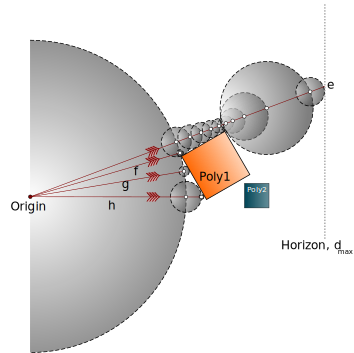
\includegraphics[width=0.75\linewidth]{images/sphere-tracing-principle}
    \caption{Illustration of the sphere tracing
      algorithm.
      Ray~\textit{e} hits no objects until reaching the horizon at
      $d_{max}$. Rays~\textit{f},~\textit{g} and~\textit{h} hit
      polygon~\textit{poly1}.}
      \label{fig:sphere-tracing-1}
\end{figure}

\newthought{Unbounding volumes} contrast with bounding volumes, which enclose a
solid. Unbounding volumes enclose a part of space without including certain
objects (whereas including means touching). For calculating a unbounding volume,
the distance between an object and the origin is being searched. Is this
distance known, it can be taken as a radius of a sphere. Sphere tracing defines
objects as implicit surfaces using distance functions. Therefore the distance
from every point in space to every other point in space and to every surface of
every object is known. These distances build a so called distance field.

\newthought{The sphere tracing algorithm} is as follows. A ray is being shot
from a viewer (an eye or a pinhole camera) through the image plane into a scene.
The radius of an unbounding volume in form of a sphere is being calculated at
the origin, as described above. This radius builds an intersection with the ray
and represents the distance, that the ray will travel in a first step. From this
intersection the next unbounding volume is being expanded and its radius is
being calculated, which gives the next intersection with the ray. This procedure
continues until an object is being hit or until a predefined maximum distance of
the ray $d_{max}$ is being reached. An object is being hit, whenever the
returned radius of the distance function is below a predefined constant
$\epsilon$. A possible implementation of the sphere tracing algorithm is shown
in~\autoref{alg:sphere-tracing}. This~\autoref{alg:sphere-tracing} is although
only showing the distance estimation. Shading is done outside, for example in a
render method which calls the sphere trace method. Shading means in this context
the determination of a surface's respectively a pixel's color.

 \begin{figure*}
   \label{alg:sphere-tracing}
   \caption{%
     An abstract implementation of the sphere tracing algorithm. Algorithm in
     pseudo code, after~\cite{hart_sphere_1994}[S. 531, Fig. 1]
   }
   \begin{pythoncode}
def sphere_trace():
    ray_distance          = 0
    estimated_distance    = 0
    max_distance          = 9001
    max_steps             = 100
    convergence_precision = 0.000001

    while ray_distance < max_distance:
        # sd_sphere is a signed distance function defining the implicit surface.
        # cast_ray defines the ray equation given the current traveled /
        # marched distance of the ray.
        estimated_distance = sd_sphere(cast_ray(ray_distance))

        if estimated_distance < convergence_precision:
            # the estimated distance is already smaller than the desired
            # precision of the convergence, so return the distance the ray has
            # travelled as we have an intersection
            return ray_distance

        ray_distance = ray_distance + estimated_distance

    # When we reach this point, there was no intersection between the ray and a
    # implicit surface, so simply return 0
    return 0
   \end{pythoncode}
\end{figure*}

\newthought{Shading} is done as proposed by~\citeauthor{whitted_improved_1980}
in~\citetitle{whitted_improved_1980}~\cite{whitted_improved_1980}. This means,
that the sphere tracing algorithm needs to return which object was hit and the
material of this object. Depending on the objects material, three cases can
occur:
\begin{enumerate*}
  \item the material is reflective and refractive,
  \item the material is only reflective or
  \item the material is diffuse.
\end{enumerate*}
For simplicity only the last case is being taken into account. For the actual
shading a local illumination method is used:~\textit{phong shading}.

\newthought{The phong illumination model} describes (reflected) light intensity
$I$ as a composition of the ambient, the diffuse and the perfect specular
reflection of a surface.

\begin{figure}
  \label{eq:phong-equation}
  \caption{The phong illumination model as defined by Phong Bui-Tuong. Note that
  the emissive term was left out intentionally as it is mainly used to achieve
  special effects.}
  \begin{equation}
    I(\vv{V}) = k_{a} \cdot L_{a} + k_{d} \displaystyle\sum_{i=0}^{n - 1} L_{i} \cdot (\vv{S_{i}} \cdot \vv{N}) + k_{s} \displaystyle\sum_{i=0}^{n - 1} L_{i} \cdot {(\vv{R_{i}} \cdot \vv{V})}^{k_{e}}
  \end{equation}
\end{figure}% -*- mode: latex; coding: utf-8 -*-

\chapter{Methodologies}
\label{chap:methodologies}

% Das Kapitel der Methoden erklärt, was (Material) untersucht wurde und wie
% (Methode) ersteres untersucht wurde. Aufgrund der Beschreibung der Methoden muss
% es möglich sein, den Versuch oder die Studie zu wiederholen. Ist die
% Beschreibung der Versuchsanordnung oder des Vorgehens von sehr geringem Umfang,
% können diese nach Rücksprache mit der Betreuungsperson auch als Absatz in der
% Einleitung oder als Unterkapitel zum Kapitel der Einleitung verfasst werden.

% Link to previous
% Make a connection to what has immediately gone before. Recap the last chapter.
% In the last chapter I showed that… Having argued in the previous chapter that…
% As a result of x, which I established in the last chapter….. It is also possible
% to make a link between this chapter and the whole argument… The first step in
% answering my research question (repeat question) .. was to.. . In the last
% chapter I …
\newthought{The last chapter} provided the fundamentals that are required for
understanding the results of this thesis.

% Focus: What does this chapter specifically do?
% Now focus the reader’s attention on what this chapter is specifically going to
% do and why it is important. In this chapter I will examine.. I will present… I
% will report … This is crucial in (aim of thesis/research question) in order to….
\newthought{This chapter} presents the methodologies that are used to implement
this thesis.

% Overview: How is it done?
% The third paragraph simply outlines the way that you are going to achieve the
% aim spelled out in the previous paragraph. It’s really just a statement of the
% contents in the order that the reader will encounter them. It is important to
% state these not simply as topics, but actually how they build up the internal
% chapter argument… I will begin by examining the definitions of, then move to
% seeing how these were applied… I first of all explain my orientation to the
% research process, positioning myself as a critical scholar.. I then explain the
% methodology that I used in the research, arguing that ethnography was the most
% suitable approach to provide answers to the question of…
\newthought{The first section of this chapter} shows a principle called literate
programming, which is used to generate this documentation and the practical
implementation in terms of a software. The second section describes the agile
methodologies, that are used to implement this thesis.

\section{Literate programming}
\label{sec:literate-programming}

\newthought{Software may be documented in different ways.} It may be in terms of
a preceding documentation, e.g. in form of a software architecture, which
describes the software conceptually and hints at its implementation. It may be
in terms of documenting the software inline through inline comments. Frequently
both methodologies are used, in independent order. However, all too frequently
the documentation is not done properly and is even neglected as it can be quite
costly with seemingly little benefit.

\newthought{Documenting software is crucial.} Whenever software is written,
decisions are made. In the moment a decision is made, it may seem intuitively
clear as it evolved by thought. This seemingly clearness of the decision is most
of the time deceptive. Is a decision still clear when some time has passed by
since making that decision? What were the facts that led to it? Is the decision
also clear for other, may be less involved persons? All these concerns show that
documenting software is crucial. No documentation at all, outdated or irrelevant
documentation can lead to unforeseen efforts concerning time and costs.

\newthought{\citeauthor{hoare-hpl-1973} states~\citeyear{hoare-hpl-1973}} in his
work~\citetitle{hoare-hpl-1973} that~\enquote{documentation must be regarded as
an integral part of the process of design and coding}~\cite[p.
195]{hoare-hpl-1973}: ~\enquote{The purpose of program documentation is to
explain to a human reader the way in which a program works so that it can be
successfully adapted after it goes into service, to meet the changing
requirements of its users, or to improve it in the light of increased knowledge,
or just to remove latent errors and oversights. The view that documentation is
something that is added to a program after it has been commissioned seems to be
wrong in principle and counter-productive in practice. Instead, documentation
must be regarded as an integral part of the process of design and coding. A good
programming language will encourage and assist the programmer to write clear
self-documenting code, and even perhaps to develop and display a pleasant style
of writing. The readability of programs is immeasurably more important than
their writeability.}~\cite[p. 195]{hoare-hpl-1973}

\newthought{Literate programming}, a paradigm proposed
in~\citeyear{knuth-lp-1984} by~\citeauthor{knuth-lp-1984}, goes even further.
\citeauthor{knuth-lp-1984} believes that \enquote{significantly better
documentation of programs} can be best achieved~\enquote{by considering programs
to be works of literature}~\cite[p.
1]{knuth-lp-1984}.~\citeauthor{knuth-lp-1984} proposes to change
the~\enquote{traditional attitude to the construction of programs}~\cite[p.
1]{knuth-lp-1984}. Instead of imagining that the main task is to instruct a
computer what to do, one shall concentrate on explaining to human beings what
the computer shall do.~\cite[p. 1]{knuth-lp-1984}

\newthought{The ideas of literate programming} have been embodied in several
software systems, the first being~\emph{WEB}, introduced
by~\citeauthor{knuth-lp-1984} himself. These systems are a combination of two
languages:
\begin{enumerate*}
  \item a document formatting language and
  \item a programming language
\end{enumerate*}.
Such a software system uses a single document as input (which can be split up in
multiple files) and generates two outputs:
\begin{enumerate*}
\item a document in a document formatting language, such as~\LaTeX{} which, may
    then be converted in a platform independent binary description, such as
    PDF.
  \item a compilable program in a programming language, such as Python or C
    which may then be compiled into an executable program.
\end{enumerate*}~\cite{knuth-lp-1984}
The first is called~\emph{weaving} and the latter~\emph{tangling}. This process
is illustrated in~\autoref{fig:weave-and-tangle}.

\begin{figure}
  \label{fig:weave-and-tangle}
  \caption{Illustration showing the processes of~\emph{weaving}
    and~\emph{tangling} documents from a input document.~\cite{knuth-lp-1984}}
  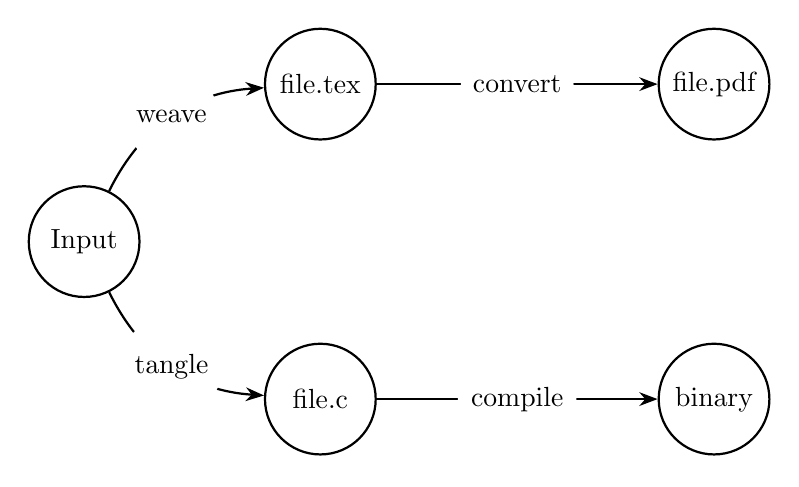
\begin{tikzpicture}
    \begin{scope}[every node/.style={minimum size=4em,circle,thick,draw}]
      \node (input) at (0,  0) {Input};
      \node (tex)   at (3,  2) {file.tex};
      \node (c)     at (3, -2) {file.c};
      \node (pdf)   at (8,  2) {file.pdf};
      \node (bin)   at (8, -2) {binary};
    \end{scope}
    \begin{scope}[>={Stealth[black]},
      every node/.style={fill=white,circle},
      every edge/.style={draw=black,thick}]
      \path [->] (input) edge[bend left=30] node {weave} (tex);
      \path [->] (input) edge[bend right=30] node {tangle} (c); 
      \path [->] (tex) edge node {convert} (pdf); 
      \path [->] (c) edge node {compile} (bin); 
    \end{scope}
  \end{tikzpicture}
\end{figure}

\newthought{Several literate programming systems were evaluated} during the
first phases of this thesis:
CWEB~\sidenote{\url{http://www-cs-faculty.stanford.edu/~uno/cweb.html}},
Noweb~\sidenote{\url{https://www.cs.tufts.edu/~nr/noweb/}},
lit~\sidenote{\url{http://cdosborn.github.io/lit/lit/root.html}},
PyLiterate~\sidenote{\url{https://github.com/bslatkin/pyliterate}},
pyWeb~\sidenote{\url{http://pywebtool.sourceforge.net/}} and
Babel~\sidenote{\url{http://orgmode.org/worg/org-contrib/babel/}} (which is part
of org mode of Emacs). All of these tools have their strengths and weaknesses.
However, none of these systems fulfill all the needed requirements:
\begin{enumerate*}
  \item Provide pretty printing of the program parts.
  \item Provide automatic references between the definition of program parts and
    their usage.
  \item Expand program parts having the same name instead of redefining them.
  \item Support Python as programming language.
  \item Allow the inclusion of files for both parts, the document formatting
    language and the programming language.
\end{enumerate*}

\newthought{Ultimately nuweb~\footnote{\url{http://nuweb.sourceforge.net/}} was
chosen} as it fulfills all these requirements. It has adapted and simplified the
ideas FunnelWeb~\footnote{\url{http://www.ross.net/funnelweb/}}. It is
independent of the programming language for the source code. As document
formatting language it uses~\LaTeX{}. Although the documentation of nuweb
states, that it has no pretty printing of source code, it provides an option to
display source code as listings. This method was modified to support visualizing
the expansion of parts as well as to use specific syntax highlighting and code
output within~\LaTeX{}.

\newthought{nuweb provides several commands to process files.} All commands
begin with an at sign (@). Whenever a file does not contain any commands the
file is copied unprocessed. The same applies for parts of files which contain no
commands. nuweb provides a single binary, which processes the
input files and generates the output files (in document formatting language and
as source code respectively). The commands are used to~\emph{specify output
files},~\emph{define fragments }and to~\emph{delimit scraps}.

\begin{table}[h]
  \caption{The major commands of nuweb.~\cite[p. 3]{briggs-nuweb-93}}
  \label{table:nuweb-commands}
  \begin{tabularx}{\textwidth}{lX}
    \toprule
    \textbf{Command} & \textbf{Description}\\
    \midrule
    \verb|@o file-name flags scrap| & \emph{Outputs} the given scrap to the
                                       defined \emph{file} using the provided
                                       flags.\\
    \verb|@d fragment-name scrap|   & Defines a~\emph{fragment} which refers to
                                       / holds the given scrap.\\
    \verb|@q fragment-name scrap|   & Defines a~\emph{quoted fragment} which refers to
                                       / holds the given scrap. Inside a quoted
                                       fragment referred fragments are not expanded.\\
    \bottomrule
  \end{tabularx}
\end{table}
\marginnote[-70pt]{Note that fragment names may be abbreviated, either during
invocation or definition. nuweb simply preserves the longest version of a
fragment name.~\cite[p. 4]{briggs-nuweb-93}}

\newthought{Scraps define content} in form of source code. They~\enquote{have
specific markers to allow precise control over the contents and
layout.}~\cite{briggs-nuweb-93} There are three ways of defining scraps, which
can be seen in~\autoref{table:nuweb-scraps}. They all include everything between
the specific markers but they differ when being typeset.
\begin{table}[h]
  \caption{Ways of defining scraps in nuweb.~\cite[p. 3]{briggs-nuweb-93}}
  \label{table:nuweb-scraps}
  \begin{tabularx}{\textwidth}{lX}
    \toprule
    \textbf{Scrap} & \textbf{Typesetting}\\
    \midrule
    \verb|@{ Content of scrap here @}| & Verbatim mode.\\
    \verb|@[ Content of scrap here @]| & Paragraph mode.\\
    \verb|@( Content of scrap here @)| & Math mode.\\
    \bottomrule
  \end{tabularx}
\end{table}

\newthought{A fragment is being invoked} by
using~\verb|@<fragment-name@>|.~\enquote{It causes the fragment fragment-name
to be expanded inline as the code is written out to a file. It is an error to
specify recursive fragment invocations.}~\cite[p. 3]{briggs-nuweb-93} There are
various other commands and details, but mentioning them would go beyond the
scope of this thesis. They can be found at~\cite{briggs-nuweb-93}.

\newthought{Literate programming can be very expressive} as all thoughts are
laid down before implementing something.~\citeauthor{knuth-lp-1984} sees this
expressiveness an advantage as one is forced to clarify his thoughts before
programming~\cite[p. 13]{knuth-lp-1984}. This is surely very true for rather
small software and partly also for larger software. The problem with larger
software is, that using literate programming, the documentation tends to be
rather large too. \emph{To overcome this aspect} the actual implementation of
the intended software is moved to the appendix~\todo{insert reference to
appendix here}.

\newthought{Another problematic aspect is the implementation of technical
details} such as imports for example or plain getter and setter methods, which
may recur and may often be very similar. While this might be interesting for
software developers or technically oriented readers, who want to grasp all the
details, this might not be interesting for other readers.~\emph{This aspect can
be overcome}, by moving recurring or seemingly uninteresting parts to a separate
file, see~\todo{add reference to code fragments}, which holds these code
fragments.

\newthought{To show the principles of literate programming} nevertheless,
without annoying the reader, only an excerpt of some details is given at this
place. One of the more interesting things of the intended software might
be the definition of a node~\todo{add reference to the node concept within
appendix} and the loading of node definitions from external files. These two
aspects are shown below. However, not all of the details are shown as this would
go beyond the scope.

\newthought{Some essential thoughts about classes and objects} may help to stay
consistent when developing the software, before implementing the node class.
Each class should at least have
\begin{enumerate}
  \item Signals --- to inform other components about events.
  \item A constructor.
  \item Various methods.
  \item Slots --- to get informed about events from other components.
\end{enumerate}
This pattern is applied to the declaration of the node class.

\newpage{}

\newthought{Implementing the node class} means simply defining a~\emph{scrap}
called~\enquote{\emph{Node definition declaration}} using the above pattern.
The~\emph{scrap} does not have any content at the moment, except references to
other scraps, which build the body of the scrap and which will be defined later
on.

\begin{figure}[h]
  \begin{flushleft} \small
\begin{minipage}{\linewidth}\label{scrap1}\raggedright\small
\NWtarget{nuweb?}{} $\langle\,${\itshape Node definition declaration}\nobreak\ {\footnotesize {?}}$\,\rangle\equiv$
\vspace{-1ex}
\begin{pythoncode}
class NodeDefinition(object):
    """Represents a definition of a node."""

    # Signals
    |\hbox{$\langle\,${\itshape Node definition signals}\nobreak\ {\footnotesize ?}$\,\rangle$}|
    |\hbox{$\langle\,${\itshape Node definition constructor}\nobreak\ {\footnotesize \NWlink{nuweb?}{?}}$\,\rangle$}|
    |\hbox{$\langle\,${\itshape Node definition methods}\nobreak\ {\footnotesize ?}$\,\rangle$}|

    # Slots
    |\hbox{$\langle\,${\itshape Node definition methods}\nobreak\ {\footnotesize ?}$\,\rangle$}||\NWsep|
\end{pythoncode}
\vspace{1.5ex}
\footnotesize
\begin{list}{}{\setlength{\itemsep}{-\parsep}\setlength{\itemindent}{-\leftmargin}}
\item {\NWtxtMacroNoRef}.

\item{}
\end{list}
\end{minipage}\vspace{4ex}
\end{flushleft}
\caption{Declaration of the node definition class.}
  \label{lst:node-def-class-decl}
\end{figure}

\vspace*{-2\baselineskip}
\newthought{The constructor} might be the first thing to implement, following
the developed pattern. In Python the constructor defines the properties of a
class~\sidenote[][-10pt]{Properties do not need to be defined in the constructor,
they may be defined anywhere within the class. However, this can lead to
confusion and it is therefore considered as good practice to define the
properties of a class in its constructor.}, therefore it defines what a class
actually is or represents --- the concept. After some thinking, and in context
of the intended software, one might come up with the properties
in~\autoref{table:node-properties} defining a node definition.

\begin{table*}[!htp]
  \begin{tabularx}{\linewidth}{lX}
    \toprule
    \textbf{Property} & \textbf{Description}\\
    \midrule
    ID          & A globally unique identifier for the node definition.          \\
    Name        & The name of the definition.                                    \\
    Description & The description of the definition. What does that definition
                  provide?                                                       \\
    Parent      & The parent object of the current node definition.              \\
    Inputs      & Inputs of the node definition. This may be distinct types or
                  references to other nodes.                                     \\
    Outputs     & The same as for inputs.                                        \\
    Invocation  & A list of the node's invocations or calls respectively.        \\
    Parts       & Defines parts that may be processed when evaluating the node.
                  Contains code which can be interpreted directly.               \\
    Connections & A list of connections of the node's inputs and outputs. Each
                  connection is composed by two parts:
                  \begin{enumerate*}
                    \item a reference to another node and
                    \item a reference to an input or an output of that node.
                  \end{enumerate*}
                  Is the reference not set, that is, its value is zero, this
                  means that the connection is internal.                         \\
    Instances   & A list of node instances from a certain node definition.       \\
    Was changed & Flag, which indicates whether a definition was changed or not. \\
    \bottomrule
  \vspace*{\baselineskip}
  \caption{Properties/attributes of the node class.}
  \label{table:node-properties}
  \end{tabularx}
\end{table*}

\newthought{Implementing the constructor} of the node definition may now follow
from the properties defined in~\autoref{table:node-properties}. As the name of
the constructor definition was already given, by using it
within~\autoref{lst:node-def-class-decl}
(\verb|@<Node definition constructor@>|), the very same name will be used for
actually defining the scrap itself.

\begin{figure}[!htbp]
  \begin{flushleft} \small
\begin{minipage}{\linewidth}\label{scrap2}\raggedright\small
\NWtarget{nuweb?}{} $\langle\,${\itshape Node definition constructor}\nobreak\ {\footnotesize {?}}$\,\rangle\equiv$
\vspace{-1ex}
\begin{pythoncode}
def __init__(self, id_):
    """Constructor.

    :param id_: the globally unique identifier of the node.
    :type  id_: uuid.uuid4
    """

    self.id_         = id_

    self.name        = ""
    self.description = ""
    self.parent      = None
    self.inputs      = []
    self.outputs     = []
    self.invocations = []
    self.parts       = []
    self.nodes       = []
    self.connections = []
    self.instances   = []
    self.was_changed = False|\NWsep|
\end{pythoncode}
\vspace{1.5ex}
\footnotesize
\begin{list}{}{\setlength{\itemsep}{-\parsep}\setlength{\itemindent}{-\leftmargin}}
\item \NWtxtMacroRefIn\ \NWlink{nuweb?}{?}.

\item{}
\end{list}
\end{minipage}\vspace{4ex}
\end{flushleft}
\caption{Constructor of the node definition class. Note that the
    identifier is given by a corresponding parameter. Identifiers have to be
    generated when defining a node using an external file.}
  \label{lst:node-def-constructor}
\end{figure}

\newthought{One of the problems mentioned before} can be seen
in~\cref{lst:node-def-constructor}: it shows a rather dull constructor
without any logic which is not interesting. Additionally importing of modules
would be needed, e.g. PyQt or system modules. This was left out deliberately.

\newthought{Node definitions will be loaded from external files} in JSON format.
This happens within the node controller component, which will not be shown here
as this would go beyond the scope. Required attributes will be mentioned
explicitly although. The method for loading the nodes,
\mintinline{python}{load_node_definitions}, defined
in~\cref{lst:load-node-definitions}, does not have any arguments. Everything
needed for loading nodes is encapsulated in the node controller.

\begin{figure}[h]
  \begin{flushleft} \small
\begin{minipage}{\linewidth}\label{scrap3}\raggedright\small
\NWtarget{nuweb?}{} $\langle\,${\itshape Load node definitions}\nobreak\ {\footnotesize {?}}$\,\rangle\equiv$
\vspace{-1ex}
\begin{pythoncode}
def load_node_definitions(self):
    """Loads all files with the ending NODES_EXTENSION
    within the NODES_PATH directory, relative to
    the current working directory.
    """|\NWsep|
\end{pythoncode}
\vspace{1.5ex}
\footnotesize
\begin{list}{}{\setlength{\itemsep}{-\parsep}\setlength{\itemindent}{-\leftmargin}}
\item \NWtxtMacroDefBy\ \NWlink{nuweb?}{?}\NWlink{nuweb?}{, ?}.
\item {\NWtxtMacroNoRef}.

\item{}
\end{list}
\end{minipage}\vspace{4ex}
\end{flushleft}
\caption{Head of the method that loads node definitions from external JSON
    files.}
  \label{lst:load-node-definitions}
\end{figure}

\vspace*{-2\baselineskip}
\newthought{When loading the node definitions}, the first thing to do is to
check whether the path containing the files with the node definitions exist or
not. Is this not the case a warning message will be logged.

\begin{figure}[!h]
  \begin{flushleft} \small
\begin{minipage}{\linewidth}\label{scrap4}\raggedright\small
\NWtarget{nuweb?}{} $\langle\,${\itshape Load node definitions}\nobreak\ {\footnotesize {?}}$\,\rangle+\equiv$
\vspace{-1ex}
\begin{pythoncode}
    if os.path.exists(self.nodes_path):
        |\hbox{$\langle\,${\itshape Load existing node definitions}\nobreak\ {\footnotesize ?}$\,\rangle$}|
    else:
        |\hbox{$\langle\,${\itshape Output warning when no node definitions are found}\nobreak\ {\footnotesize \NWlink{nuweb29}{29}}$\,\rangle$}||\NWsep|
\end{pythoncode}
\vspace{1.5ex}
\footnotesize
\begin{list}{}{\setlength{\itemsep}{-\parsep}\setlength{\itemindent}{-\leftmargin}}
\item \NWtxtMacroDefBy\ \NWlink{nuweb?}{?}\NWlink{nuweb?}{, ?}.
\item {\NWtxtMacroNoRef}.

\item{}
\end{list}
\end{minipage}\vspace{4ex}
\end{flushleft}
\caption{Check whether the path containing the node definition files exist or
    not.}
  \label{lst:nodes-controller-load-nodes-2}
\end{figure}

\newthought{Literate programming allows great verbosity} as can be seen
in~\cref{lst:nodes-controller-load-nodes-2}. Logging the warning message is
simply a matter of preparing a corresponding message and calling
the~\mintinline{python}{fatal} method of the logging interface.

\begin{figure}[!h]
  \caption{Output a warning when the path containing the node definition files
    does not exist.}
  \label{lst:nodes-controller-load-nodes-3}
  \begin{flushleft} \small
\begin{minipage}{\linewidth}\label{scrap5}\raggedright\small
\NWtarget{nuweb29}{} $\langle\,${\itshape Output warning when no node definitions are found}\nobreak\ {\footnotesize {29}}$\,\rangle\equiv$
\vspace{-1ex}
\begin{pythoncode}
    message = QtCore.QCoreApplication.translate(
        __class__.__name__,
        "No files with node definitions found at %s." % self.nodes_path
    )
    self.logger.fatal(message)|\NWsep|
\end{pythoncode}
\vspace{1.5ex}
\footnotesize
\begin{list}{}{\setlength{\itemsep}{-\parsep}\setlength{\itemindent}{-\leftmargin}}
\item \NWtxtMacroRefIn\ \NWlink{nuweb?}{?}.

\item{}
\end{list}
\end{minipage}\vspace{4ex}
\end{flushleft}
\end{figure}

\section{Agile software development}
\label{sec:agile-software-development}

TBD.% -*- mode: latex; coding: utf-8 -*-

\chapter{Results}
\label{chap:results}

\todo[inline]{Write chapter.}

% Gestützt auf Quellen, Messungen und Datenerhebungen werden die anhand der
% Fragestellung gewon- nenen Ergebnisse präsentiert [3, p. 116]. Während das
% Kapitel zu Material und Methoden ( 3.2.3) oder das entsprechende Unterkapitel
% der Einleitung die Versuchsanordnung beschreibt, werden im Kapitel Ergebnisse
% der Versuchsablauf mit den Resultaten objektiv wiedergegeben. Alle Überlegungen,
% Berechnungen oder Experimente des Berichts müssen vollständig nachvollziehbar
% sein [3, p. 26]. Zusammen mit der Diskussion und den Folgerungen machen die
% Ergebnisse qualitativ und quantitativ den Hauptteil des Berichts aus [3, p. 26].

% Resultate weniger kritisch, erst in Diskussion, überlappt sich aber.% -*- mode: latex; coding: utf-8 -*-

\chapter{Discussion and conclusion}
\label{chap:discussion-conclusion}

\todo[inline]{Write chapter.}

% Im Kapitel Diskussion setzt sich die Autorin, der Autor mit den erzielten
% Ergebnissen auseinander. Diese werden interpretiert und mit Erkenntnissen aus
% anderen Studien zur gleichen Fragestellung beurteilt. Die Diskussion schafft die
% nötigen Grundlagen, damit die in der Einleitung formulierte Fragestellung
% möglichst gut und sachlich richtig beantwortet werden kann.

% In den Folgerungen können die wichtigsten Ergebnisse in ihrer kritischen
% Würdigung prägnant zusammengefasst werden. Es wird eine Art Schlussbilanz
% gezogen. Aus der detaillierten Darstellung der Ergebnisse und deren Diskussion
% lässt sich in der Regel eine Antwort auf die Ausgangsfrage ableiten [3, p. 26].
% Die Antwort auf die Fragestellung kann zu Empfeh- lungen für die Ausführung in
% der Praxis oder für weitere Studien führen. Die Folgerungen dürfen keine neuen
% Elemente und Aspekte enthalten, welche nicht schon in den Ergebnissen und in der
% Diskussion behandelt wurden. Wenn die Problemstellung der Arbeit nur sehr wenige
% Folgerungen verlangt, können diese auch als Schlussteil in die Diskussion
% integriert werden.
% TODO: Check if still needed
% i inc/procedure.w
% i inc/implementation.w


% Backmatter
%---------------------------------------------------------------------------
\backmatter{}

% Appendix
% i inc/appendix.w
\todo[inline]{fix appendix}

% Bibliography
\printbibliography{}

% Glossary
% \cleardoublepage{}
% \phantomsection{}
% \addcontentsline{toc}{chapter}{Glossary}
% \glsaddall{}
% \printglossaries{}
\todo[inline]{Fix glossaries}

% Index
% \printindex{}
\todo[inline]{Print index}

\end{document}
